\section{The preceptron}

\subsection*{Problem 5}

\[
w_{k+1}=\begin{cases}
w_{k}+x_{k} & if\, t_{k}=+1\\
w_{k}-x_{k} & if\, t_{k}=-1
\end{cases}
\]
\[
b_{k+1}=\begin{cases}
b_{k}+1_{k} & if\, t_{k}=+1\\
b_{k}-1_{k} & if\, t_{k}=-1
\end{cases}
\]


\subsection*{Problem 7}
\[
\tilde{w}^{T}w_{k}=\tilde{w}^{T}\left(w_{k-1}+t_{k-1}x_{k-1}\right)=\tilde{w}^{T}\left(w_{k-2}+t_{k-2}x_{k-2}+t_{k-1}x_{k-1}\right)
\]
\[
\tilde{w}^{T}w_{k}=\tilde{w}^{T}\sum_{i=0}^{k-1}t_{i}w_{i}
\]
\[
\tilde{w}^{T}w_{k}=\sum_{i=0}^{k-1}t_{i}\tilde{w}^{T}w_{i}
\]
by knowing that $t_{i}\tilde{w}^{T}w_{i}\geq k\gamma$ we can assert
the following
\[
\tilde{w}^{T}w_{k}=\sum_{i=0}^{k-1}t_{i}\tilde{w}^{T}w_{i}\geq k\gamma
\]

\newpage
\subsection*{Problem 6}
\begin{figure}
\centering{}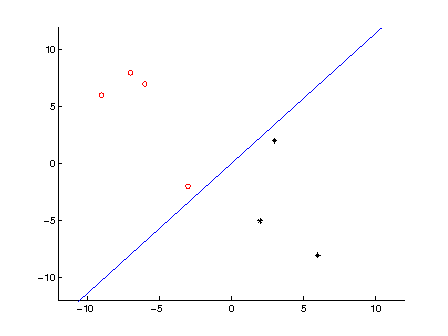
\includegraphics[width=1\textwidth]{plots/6_1}\caption{Problem 6 step 1}
\end{figure}
\begin{figure}
\centering{}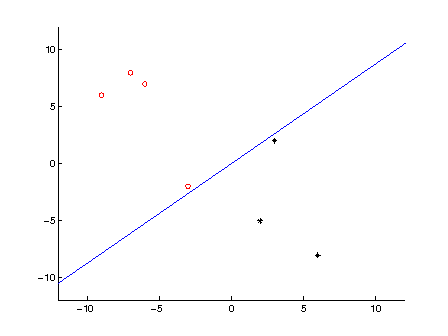
\includegraphics[width=1\textwidth]{plots/6_2}\caption{Problem 6 step 2}
\end{figure}
\begin{figure}
\centering{}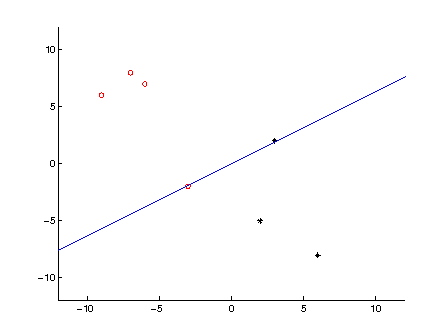
\includegraphics[width=1\textwidth]{plots/6_3}\caption{Problem 6 step 3}
\end{figure}
\begin{figure}
\centering{}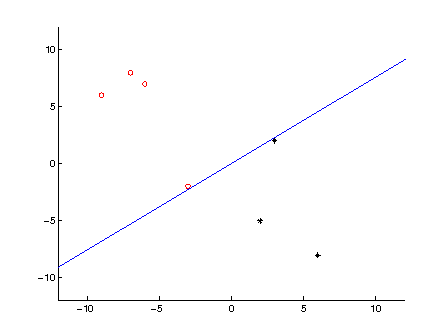
\includegraphics[width=1\textwidth]{plots/6_4}\caption{Problem 6 step 4}
\end{figure}
\begin{figure}
\centering{}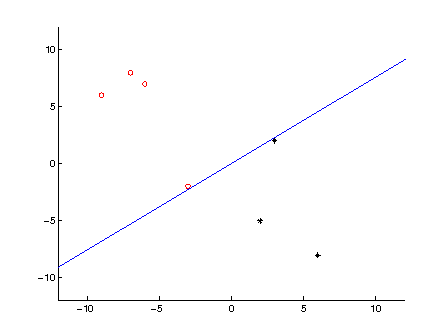
\includegraphics[width=1\textwidth]{plots/6_4}\caption{Problem 6 step 5}
\end{figure}
\begin{figure}
\centering{}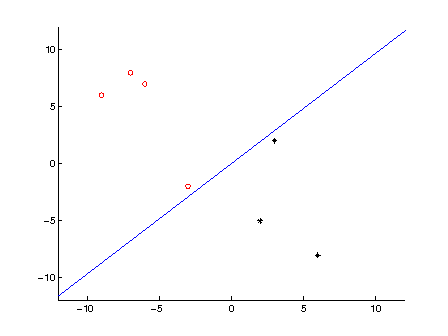
\includegraphics[width=1\textwidth]{plots/6_6}\caption{Problem 6 step 6}
\end{figure}
\begin{figure}
\centering{}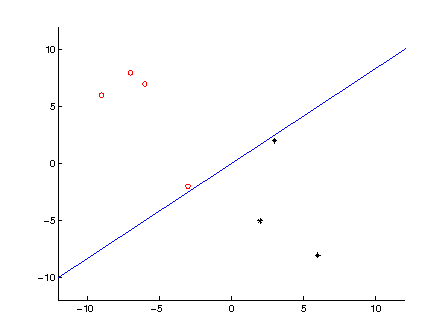
\includegraphics[width=1\textwidth]{plots/6_7}\caption{Problem 6 step 7}
\end{figure}
